\documentclass[fr]{../../../../../../eplexam}
\usepackage{ulem}

\setlength\parindent{0pt}

\renewcommand{\b}[1]{\mathbf{#1}}
\newcommand{\tend}[1]{\oalign{\mbox{\boldmath$#1$}\crcr\hidewidth$\scriptscriptstyle\sim$\hidewidth}}
\renewcommand{\vec}[1]{\uline{#1}}
\newcommand{\matr}[1]{\uuline{#1}}
\DeclareMathOperator{\Difff}{D}
\newcommand{\Dif}{\Difff\!}
\newcommand{\fDif}[2]{\dfrac{\Dif #1}{\Dif #2}}
\DeclareMathOperator{\customgrad}{grad}
\renewcommand{\grad}{\customgrad}


\hypertitle{Mécanique des milieux continus}{5}{MECA}{1901}{2019}{Janvier}{Mineure}
{Nathan Jacques \and Béatrice Desclée \and Thomas Pomponio}
{Issam Doghri et Philippe Chatelain}


\section{Théorie ID}

\subsection{Vrai ou faux, justifier}

Soient $\matr{C} = \matr{F}^T \cdot \matr{F}$, $\matr{D}$ le tenseur taux de déformation et $\fDif{}{t}$ la dérivée particulaire,

\begin{enumerate}
  \item $\fDif{\matr{C}}{t} = \matr{F}^T  \cdot  \matr{D}  \cdot  \matr{F}$
  \item $\fDif{}{t}(\text{tr}\matr{C}) = \text{tr} \left( \fDif{\matr{C}}{t} \right)$
  \item $\fDif{}{t}(\text{det}\matr{C}) = \text{det} \left( \fDif{\matr{C}}{t} \right)$
\end{enumerate}

\subsection{Notations}

On donne l'équation aux dérivées partielles suivante (dite de Cahn-Hilliard et qui décrit un changement de phase):

\[
\frac{\partial c}{\partial t} = f(\vec{x},t) - \nabla  \cdot  \left\{ -\matr{M}  \cdot  \nabla \left[ g(c) - \nabla  \cdot  \left( \matr{K}  \cdot  \nabla c \right) \right] \right\}
\]

où $c(\vec{x},t)$ désigne la concentration des phases, $f(\vec{x},t)$ est un terme source, $\matr{M}(\vec{x},t)$ et $\matr{K}(\vec{x},t)$ sont des tenseurs d'ordre 2 symétriques (modélisant respectivement la mobilité et l'énergie d'interface).

\begin{enumerate}
  \item Réécrire cette équation en utilisant la notation indicielle en coordonnées
  cartésiennes
  \item Réécrire le résultat du point 1 dans le cas suivant: $K_{ij} = k(t)\delta_{ij}$
  et $M_{ij} = m(t)\delta_{ij}$
  \item Réécrire le résultat du point 2 en utilisant uniquement le Laplacien dans
  les dérivées spatiales
\end{enumerate}

%-------------------------------------------------------------------------%
% DEBUT SOLUTION QUESTION 1 %
%-------------------------------------------------------------------------%

\begin{solution}

\textbf{Réponse sous-question 1.1.1 :} FAUX.

Réponse correcte : $\fDif{\matr{E}}{t}=\matr{F}^T.\matr{D} \cdot \matr{F}$.

On s'intéresse à la quantité $\vec{\dif{x}} \cdot \vec{\dif{x}}' - \vec{\dif{x}} \cdot \vec{\dif{x}}$ et à sa dérivée particulaire :

\begin{equation*}
\begin{split}
	\fDif{}{t} \left( \vec{\dif{x}} \cdot \vec{\dif{x}}' - \vec{\dif{x}} \cdot \vec{\dif{x}}' \right) & = \fDif{}{t} \left( \vec{\dif{x}} \cdot \vec{\dif{x}}' \right) \\
 	& = \fDif{\vec{\dif{x}}}{t} \cdot \vec{\dif{x}}' + \vec{\dif{x}} \cdot \fDif{\vec{\dif{x}}}{t} \\
 	& = ( \matr{\grad} \ \vec{V} ) \cdot \vec{\dif{x}} \cdot \vec{\dif{x}}' + \vec{\dif{x}} \cdot ( \matr{\grad} \ \vec{V} ) \cdot \vec{\dif{x}}' \\
 	& = \vec{\dif{x}} \cdot ( \matr{\grad} \ \vec{V} )^T \cdot \vec{\dif{x}}' + \vec{\dif{x}} \cdot (\matr{grad} \ \vec{V}) \cdot \vec{\dif{x}}' \\
 	& = \vec{\dif{x}} \cdot \left[(\matr{\grad} \ \vec{V}) + (\matr{\grad} \ \vec{V})^T \right] \cdot \vec{\dif{x}}' \\ 
 	& = 2 \ \vec{\dif{x}} \cdot \matr{D} \cdot \vec{\dif{x}}'
\end{split}
\end{equation*}

Ou encore :

\begin{equation*}
\begin{split}
\fDif{}{t}(\vec{\dif{x}} \cdot \vec{\dif{x}}' - \vec{\dif{x}} \cdot \vec{\dif{x}}')
& = \fDif{}{t}(\matr{F} \cdot \vec{\dif{x}} \cdot \matr{F} \cdot \vec{\dif{x}}' - \vec{\dif{x}} \cdot \vec{\dif{x}}') \\
& = \fDif{}{t}(\vec{\dif{x}} \cdot \matr{F}^T \cdot \matr{F} \cdot \vec{\dif{x}}' - \vec{\dif{x}} \cdot \vec{\dif{x}}') \\
& = \fDif{}{t}(\vec{\dif{x}} \cdot \matr{C} \cdot \vec{\dif{x}}' - \vec{\dif{x}} \cdot \matr{I} \cdot \vec{\dif{x}}') \\
& = \fDif{}{t} \left[ \vec{\dif{x}} \cdot (\matr{C}-\matr{I}) \cdot \vec{\dif{x}}' \right] \\
& = \fDif{}{t} \left[ \vec{\dif{x}} \cdot (\matr{C}-\matr{I}) \cdot \vec{\dif{x}}' \right] \\
& = \fDif{}{t}(\vec{\dif{x}} \cdot 2 \ \matr{E} \cdot \vec{\dif{x}}') \\
& = 2 \ \vec{\dif{x}} \cdot \fDif{\matr{E}}{t} \cdot \vec{\dif{x}}' 
\end{split}
\end{equation*}

Donc, $\fDif{\matr{E}}{t}=\matr{F}^T \cdot \matr{D} \cdot \vec{F}$.


\textbf{Réponse sous-question 1.1.2 :} VRAI.

Membre de gauche : $\fDif{}{t} (tr \ \matr{C}) = \fDif{C_{11}}{t}$

Membre de droite : $\left(\fDif{\matr{C}}{t} \right)_{ij} = \fDif{C_{ij}}{t}$ => $tr \left(\fDif{\matr{C}}{t} \right) = \left( \fDif{\matr{C}}{t} \right)_{ll} = \fDif{C_{11}}{t} = \fDif{}{t} (tr \ \matr{C})$

\textbf{Réponse sous-question 1.1.3 :} FAUX.

Membre de gauche : 

\begin{equation*}
\begin{split}
\fDif{}{t}(det \matr{C}) & = \fDif{}{t}(e_{ijk} \ C_{1i} \ C_{2j} \ C_{3k}) \\
& = e_{ijk} \ \fDif{C_{1i}}{t} \ C_{2j} \ C_{3k} +  e_{ijk} \  C_{1i} \fDif{C_{2j}}{t} \ C_{3k} + e_{ijk} \ C_{1i} \ C_{2j} \ \fDif{C_{3k}}{t}
\end{split}
\end{equation*}

Membre de droite : 

\begin{equation*}
\begin{split}
det \left( \fDif{\matr{C}}{t} \right) & = e_{ijk} \ \left( \fDif{\matr{C}}{t} \right)_{i1} \ \left( \fDif{\matr{C}}{t} \right)_{j2} \ \left( \fDif{\matr{C}}{t} \right)_{k3} \\ 
& = e_{ijk} \ \fDif{C_{i1}}{t} \ \fDif{C_{2j}}{t} \ \fDif{C_{3k}} {t}
\end{split}
\end{equation*}

\textbf{Réponse sous-question 1.2.1}

\begin{equation*}
\begin{split}
\frac{\partial c}{\partial t} & = f(\vec{x},t) - \text{\text{div}} \left\{ - \matr{M} \cdot \vec{\grad} \ \left[ g(c) - \text{\text{div}} \left( \matr{K} \cdot \vec{\grad} \ c \right) \right] \right\} \\
& = f(\vec{x},t) - \frac{\partial}{\partial x_i} \left\{ - \matr{M} \cdot \vec{\grad} \  \left[ g(c) - \text{\text{div}} \left( \matr{K} \cdot \vec{\grad} \ c \right) \right] \right\}_i \\
& = f(\vec{x},t) - \frac{\partial}{\partial x_i} \left\{ -M_{ij} \ \left\{\vec{\grad} \  \left[ g(c) - \text{\text{div}} \ \left( \matr{K} \ \cdot \ \vec{\grad} \ c \right) \right] \right\}_j \right\} \\
& = f(\vec{x},t)-\frac{\partial}{\partial x_i} \left\{-M_{ij} \ \frac{\partial}{\partial x_j} \left[ g(c) - \frac{\partial}{\partial x_k} \left( \matr{K}\ \cdot \ \vec{\grad}  \ c \right)_k \right] \right\}  \\
& = f(\vec{x},t) - \frac{\partial}{\partial x_i} \left\{-M_{ij} \ \frac{\partial}{\partial x_j} \left[ g(c) - \frac{\partial}{\partial x_k} \left(K_{kl} \ \frac{\partial c}{\partial x_l} \right) \right] \right\}
\end{split}
\end{equation*}

\textbf{Réponse sous-question 1.2.2}

\begin{equation*}
\begin{split}
\frac{\partial c}{\partial t} & = f(\vec{x},t) - \frac{\partial}{\partial x_i} \left\{-M_{ij} \ \frac{\partial}{\partial x_j} \left[ g(c) - \frac{\partial}{\partial x_k} \left(K_{kl} \ \frac{\partial c}{\partial x_l} \right) \right] \right\} \\
& = f(\vec{x},t) - \frac{\partial}{\partial x_i} \ \left\{ -m(t) \ \delta_{ij} \ \frac{\partial}{\partial x_j} \left[g(c)-\frac{\partial}{\partial x_k} \left(k(t) \delta_{kl} \ \frac{\partial c}{\partial x_l} \right) \right] \right\} \\ 
& = f(\vec{x},t) + m(t) \frac{\partial}{\partial x_i} \left\{ \frac{\partial}{\partial x_i} \left[g(c)-k(t) \frac{\partial}{\partial x_k} \left(\frac{\partial c}{\partial x_k} \right) \right] \right\}  \\
& = f(\vec{x},t) + m(t) \frac{\partial^2}{\partial x_i^2} \left[g(c)-k(t) \frac{\partial^2 c}{\partial x_k^2} \right] \\
& = f(\vec{x},t) + m(t) \frac{\partial^2g(c)}{\partial x_i^2} - m(t) \ k(t) \frac{\partial^2}{\partial x_i^2} \left( \frac{\partial^2 c}{\partial x_k^2} \right) 
\end{split}
\end{equation*}

\textbf{Réponse sous-question 1.2.3}

\begin{equation*}
\begin{split}
\frac{\partial c}{\partial t} & = f(\vec{x},t) + m(t) \frac{\partial^2g(c)}{\partial x_i^2} - m(t) \ k(t) \frac{\partial^2}{\partial x_i^2} \left( \frac{\partial^2 c}{\partial x_k^2} \right)   \\
& = f(\vec{x},t)+m(t) \ \Delta \left(g(c)\right)-m(t) \ k(t) \ \Delta \left(\Delta c \right) 
\end{split}
\end{equation*}

\textit{NdC : je ne suis pas certain que la dernière ligne de chacune des trois réponses soit assez développée : doit-on expliciter le fait que $c$ est une fonction de $\vec{x}$ et, pour les dérivées et le laplacien de $g(c)$, écrire une dérivée en chaîne ?}

\end{solution}

%-------------------------------------------------------------------------%
% FIN SOLUTION QUESTION 1 %
%-------------------------------------------------------------------------%

\section{Théorie PC}
\subsection{} En bref, qu'énonce le théorème de Green-Naghdi-Rivlin? Expliquez
\textbf{brièvement} comment le prouver.
\subsection{} Comment avons-nous étudié une discontinuité des champs se déplaçant
au sein d'un milieu continu? Appliquer ce traitement à la conservation de la quantité
de mouvement et donner un exemple physique où cette relation peut être utile.

\nosolution

\section{Application Solide: Cisaillement simple d'un solide hyper-élastique}
Soient $J = \text{det}\matr{F}$, $\matr{C} = \matr{F}^T  \cdot  \matr{F}$ et $\matr{B} = \matr{F}  \cdot  \matr{F}^T$, un modèle hyper-élastique (dit \og neo-Hookean \fg{}) est défini comme suit:
\[
\tend{\sigma} = \frac{1}{J} \matr{F}  \cdot  \left\{ \mu (\text{det}\matr{C})^{-1/3} \matr{1} + \left[ \kappa \left( \text{det}\matr{C} - \sqrt{\text{det}\matr{C}} \right) - \frac{\mu}{3} (\text{det}\matr{C})^{-1/3} \text{tr}\matr{C} \right] \matr{C}^{-1} \right\}  \cdot  \matr{F}^T
\]
où $\kappa >0$ et $\mu >0$ des constantes matérielles.

\begin{enumerate}
  \item Exprimer $\matr{\sigma}$ en fonction de $\matr{B}$ (et ses invariants), de $\kappa$ et de $\mu$ uniquement;
  \item Exprimer la trace de $\matr{\sigma}$ en fonction de $\kappa$ et $J$ uniquement;
  \item Montrer que la partie déviatorique de $\matr{\sigma}$ est donnée par:
  \[
  \text{dev}(\matr{\sigma}) = \mu  \ f(J) \ \text{dev} \ (\matr{B})
  \]
  où $f$ est une fonction quelconque de $J$.
\end{enumerate}

On considère un solide initialement cubique (de côté $L_0$ et occupant l'espace $0\leq X_1,X_2,X_3\leq L_0$) soumis à une transformation dite de cisaillement simple qui est décrite comme suit dans un repère orthonormé fixe $(O,\hat{e}_1,\hat{e}_2,\hat{e}_3)$:
\[
x_1 = X_1 + \gamma (t)X_2 \quad ; \quad x_2=X_2 \quad ; \quad x_3 = X_3
\]
où $\gamma (t)$ est une fonction continue et dérivable qui vérifie
\[
\gamma (0)=0 \quad ; \quad \gamma (t) > 0\,, \quad \forall t>0
\]

\begin{enumerate}
  \item Calculer les matrices représentant $\matr{F},\matr{B}$ et le tenseur de Green-Lagrange;
  \item Calculer la matrice représentant $\matr{\sigma}$. Commentez.
  \item Que devient la facette initialement en $X_2 = L_0$? Calculer et représenter graphiquement les composantes normales et tangentielles des forces de contact surfaciques qui s'exercent sur la facette déformée. Commentez.
  \item Idem pour la facette initialement en $X_1 = L_0$.
  \item Calculer les contraintes principales.
  \item Dessiner les cercles de Mohr et calculer la contrainte de cisaillement maximale.
  \item Dans le cas de petites déformations, $\gamma (t)$ est petite et on néglige $(\gamma (t))^2$ ainsi que les termes d'ordre supérieur devant 1. Que deviennent les résultats de 1 à 6 dans ce cas? Quel est le lien avec l'élasticité linéaire et isotrope? Que signifient $\mu$ et $\kappa$?
\end{enumerate}

%-------------------------------------------------------------------------%
% DEBUT SOLUTION QUESTION 3 %
%-------------------------------------------------------------------------%

\begin{solution}

\textit{NdC : lors de l'examen, l'assistant à dit qu'il n'était pas nécessaire de répondre à la première partie (questions 1 à 3) pour pouvoir faire la suite de l'exercice (questions 1 à 7), mais que ça pouvait simplifier les calculs.  Je n'ai pas trouvé les réponses pour la première partie lors de l'examen en janvier, ni en le refaisant en août ...  Je ne peux que proposer une solution pour la seconde partie.  Pour la seconde partie, la photo de la feuille avec les solutions d'un assistant a été postée sur Facebook.  Les solutions que je propose ici sont les mêmes, sauf pour quelques points.  Je n'ai pas trouvé comment obtenir les solutions de l'assistant.  Pour ces points-là, j'ai 1) laissé mon raisonnement et ma solution, 2) indiqué la solution de l'assistant et 3) mis un commentaire pour attirer votre attention.  J'espère que quelqu'un pourra trouver les raisonnements qui mènent aux bonnes solutions et corriger ce que je propose.}

R\textbf{éponse partie 2, sous-question 1}

$\vec{x} = \begin{pmatrix} X_1 \ + \ \gamma(t) \ X_2 \\ X_2 \\ X_3 \end{pmatrix}$

$\matr{F} = \frac{\partial \vec{x}}{\partial \vec{X}} = \begin{pmatrix} 1 & \gamma & 0 \\ 0 & 1 & 0 \\ 0 & 0 & 1 \end{pmatrix}$

$\matr{B} = \matr{F} \cdot \matr{F}^T = \begin{pmatrix} 1 & \gamma & 0 \\ 0 & 1 & 0 \\ 0 & 0 & 1 \end{pmatrix} \ \begin{pmatrix} 1 & 0 & 0 \\ \gamma & 1 & 0 \\ 0 & 0 & 1 \end{pmatrix} \ = \ \begin{pmatrix} 1+\gamma^2 & \gamma & 0 \\ \gamma & 1 & 0 \\ 0 & 0 & 1 \end{pmatrix}$

$\matr{E} = \frac{1}{2} \left(\matr{C} - \matr{I} \right) = \ \begin{pmatrix} 0 & \frac{\gamma}{2} & 0 \\ \frac{\gamma}{2} & \frac{\gamma^2}{2} & 0 \\ 0 & 0 & 0 \end{pmatrix}$

\textbf{Réponse partie 2, sous-question 2}

Il faut utiliser la loi de comportement donnée au début de l'énoncé.  On a déjà calculé $\matr{F}$.  On commence par calculer les autres termes :

$\matr{C} = \matr{F} \cdot \matr{F}^T = \begin{pmatrix} 1 & 0 & 0 \\ \gamma & 1 & 0 \\ 0 & 0 & 1 \end{pmatrix} \ \begin{pmatrix} 1 & \gamma & 0 \\ 0 & 1 & 0 \\ 0 & 0 & 1 \end{pmatrix} \  = \ \begin{pmatrix} 1 & \gamma & 0 \\ \gamma & 1+\gamma^2 & 0 \\ 0 & 0 & 1 \end{pmatrix}$

$\text{det} \ \matr{C} = (1 \ + \ \gamma^2) - \gamma^2 = 1$

$\text{tr} \ \matr{C} = 3 \ + \ \gamma^2$

$\matr{C}^{-1} = \frac{1}{J} \ \begin{pmatrix} 1+\gamma^2 & -\gamma & 0  \\  -\gamma & 1 & 0  \\  0 & 0 & 1 \end{pmatrix}^{T} = \begin{pmatrix} 1+\gamma^2 & -\gamma & 0  \\  -\gamma & 1 & 0  \\  0 & 0 & 1 \end{pmatrix}$

$J = \text{det} \ \matr{F} = 1$

\textit{NdC : il faut maintenant injecter tout ça dans la loi de comportement.  Il me semble plus facile de distribuer $\matr{F}$ et $\matr{F}^T$ dans les crochets, de traiter les deux termes de la somme séparément et puis de les additionner, plutôt que de calculer le terme entre crochets puis de le multiplier avec $\matr{F}$ et $\matr{F}^T$.  Si on calcule d'abord le terme entre crochet, on obtient une matrice dont certains éléments sont la somme de plusieurs termes.  Et lorsque l'on multiplie ensuite cette matrice avec $\matr{F}$ et $\matr{F}^T$, ça devient pénible (testé à l'examen de janvier ...).  Mais si on commence par traiter les deux membres séparément, on obtient deux matrices assez simple qu'il suffit d'additionner (testé en révisant en août ...).}

En distribuant $\matr{F}$ et $\matr{F}^T$ sur le premier terme de la somme, on obtient :

\begin{equation*}
\begin{split}
\matr{\sigma}_1 & = \frac{1}{J} \ \matr{F} \cdot \left\{ \mu \ (\text{det} \matr{C})^{-1/3} \ \matr{I} \right\} \cdot \matr{F}^T  \\
& = \mu \ \matr{F} \cdot \matr{I} \cdot \matr{F}^T  \\
& = \mu \ \matr{B}
\end{split}
\end{equation*}

En distribuant $\matr{F}$ et $\matr{F}^T$ sur le second terme de la somme, on obtient :

\begin{equation*}
\begin{split}
\matr{\sigma}_2 & = \frac{1}{J} \matr{F} \cdot \left\{ \left[ \kappa \left( \text{det} \matr{C} - \sqrt{\text{det} \matr{C}} \right) -\frac{\mu}{3} \left(\text{det} \matr{C} \right)^{-1/3} \text{tr} \matr{C} \right] \matr{C}^{-1} \right\}  \cdot  \matr{F}^T  \\
& = \matr{F}  \cdot  \left[ \ - \frac{\mu}{3} \ (3+\gamma)^2 \ \matr{C}^{-1} \right]  \cdot  \matr{F}^T  \\
& = \frac{-\mu \ (3+\gamma)^2}{3} \ 
    \begin{pmatrix} 1 & \gamma & 0 \\ 0 & 1 & 0 \\ 0 & 0 & 1 \end{pmatrix} \
    \begin{pmatrix} 1+\gamma^2 & -\gamma & 0 \\ -\gamma & 1 & 0 \\ 0 & 0 & 1 \end{pmatrix}
    \begin{pmatrix} 1 & 0 & 0 \\ \gamma & 1 & 0 \\ 0 & 0 & 1 \end{pmatrix}  \\
& = \frac{-\mu \ (3+\gamma)^2}{3} \ 
    \begin{pmatrix} 1 & \gamma & 0 \\ 0 & 1 & 0 \\ 0 & 0 & 1 \end{pmatrix} \
    \begin{pmatrix} 1 & -\gamma & 0 \\ 0 & 1 & 0 \\ 0 & 0 & 1 \end{pmatrix}  \\
& = \frac{-\mu \ (3+\gamma)^2}{3} \ \begin{pmatrix} 1 & 0 & 0 \\ 0 & 1 & 0 \\ 0 & 0 & 1 \end{pmatrix} \\ 
& = \frac{-\mu \ (3+\gamma)^2}{3} \ \matr{I}
\end{split}
\end{equation*}

En regroupant, on obtient $\matr{\sigma}$ :

$\matr{\sigma} = \mu \ \matr{B} - \frac{\mu \ (3+\gamma)^2}{3} \ \matr{I} = \mu \ \left[ \matr{B}-\frac{\mu \ (3+\gamma)^2}{3} \ \matr{I} \right] = \begin{pmatrix} \frac{2 \mu {\gamma}^2}{3} & \mu \gamma & 0 \\ \mu \gamma & -\frac{\mu  {\gamma}^2}{3} & 0 \\ 0 & 0 & -\frac{\mu {\gamma}^2}{3} \end{pmatrix}$

Commentaire : $\matr{\sigma}$ est bien symmétrique.

\textbf{Réponse partie 2, sous-question 3}

Comme à la question suivante il faut traiter une autre facette, on peut regarder directement comment le volume se déforme.    On peut le voir en calculant la position des sommets dans la configuration actuelle :

\begin{center}
\begin{tabular}{|c|c|c|c|c|c|c|c|c|}
  \hline
  \rule{0pt}{40pt} $\vec{X}$
  & $\begin{pmatrix} 0 \\ 0 \\ 0 \end{pmatrix}$
  & $\begin{pmatrix} L_0 \\ 0 \\ 0 \end{pmatrix}$
  & $\begin{pmatrix} L_0 \\ L_0 \\ 0 \end{pmatrix}$
  & $\begin{pmatrix} 0 \\ L_0 \\ 0 \end{pmatrix}$
  & $\begin{pmatrix} 0 \\ 0 \\ L_0 \end{pmatrix}$
  & $\begin{pmatrix} L_0 \\ 0 \\ L_0 \end{pmatrix}$
  & $\begin{pmatrix} L_0 \\ L_0\\  L_0 \end{pmatrix}$
  & $\begin{pmatrix} 0 \\  L_0 \\ L_0 \end{pmatrix}$ \\
  \hline 
  \rule{0pt}{40pt} $\vec{x}$
  & $\begin{pmatrix} 0 \\ 0 \\ 0 \end{pmatrix}$ 
  & $\begin{pmatrix} L_0 \\ 0 \\ 0 \end{pmatrix}$
  & $\begin{pmatrix} L_0+L_0\gamma \\ L_0 \\ 0 \end{pmatrix}$
  & $\begin{pmatrix} L_0\gamma \\ L_0 \\ 0 \end{pmatrix}$
  & $\begin{pmatrix} 0 \\ 0 \\  L_0 \end{pmatrix}$
  & $\begin{pmatrix} L_0 \\ 0 \\ L_0 \end{pmatrix}$
  & $\begin{pmatrix} L_0+L_0\gamma \\ L_0 \\ L_0 \end{pmatrix}$
  & $\begin{pmatrix} L_0\gamma \\ L_0 \\ L_0 \end{pmatrix}$ \\ 
  \hline
\end{tabular}
\end{center}

Le cube se déforme donc de la manière suivante (au crayon : configuration initiale, en rouge : configuration actuelle, ou déformée) :

\begin{center}
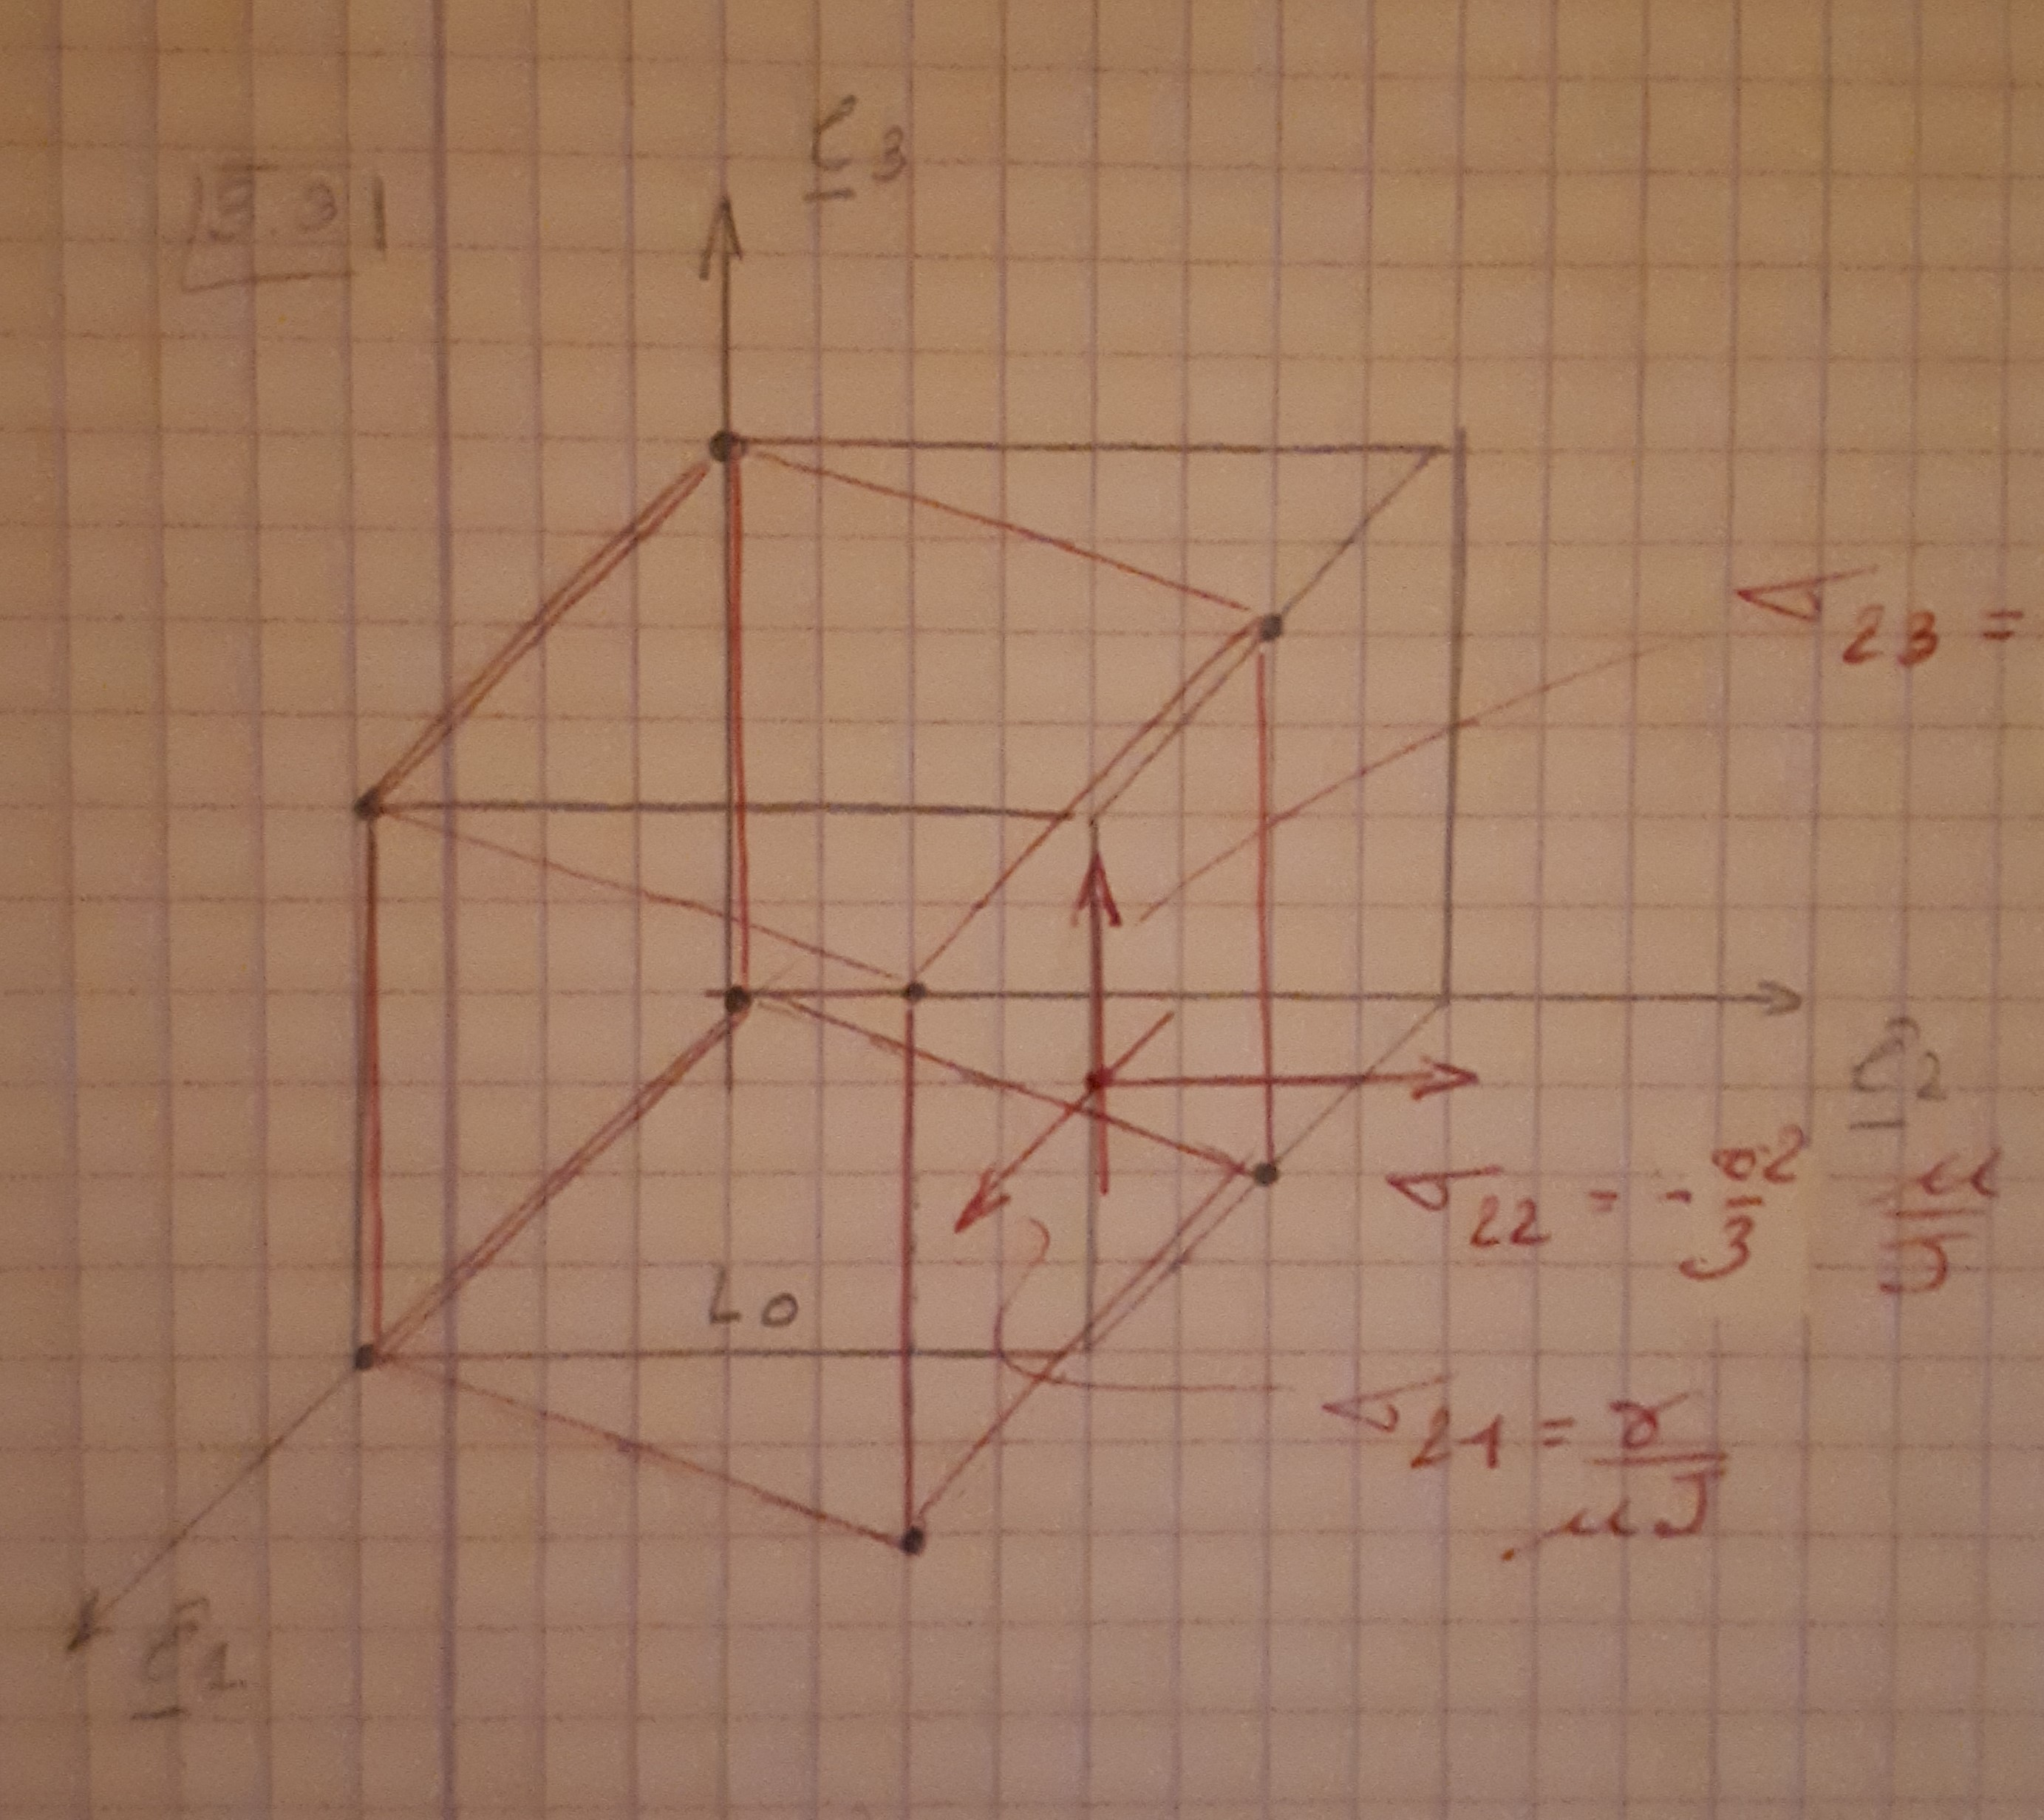
\includegraphics[width=0.5\textwidth]{MMC_Janvier_2019_Min_Q3_Image1.jpg}
\end{center}

La facette en $X_2=L_0$ est translatée de $\gamma L_0$ dans la direction $\vec{\hat{e}}_1$ et son orientation ne change pas : sa normale sortante reste $\vec{\hat{e}}_2$.

Contrainte sur la facette : $\vec{T}(\vec{\hat{n}} = \vec{\hat{e}}_2) = \matr{\sigma}  \cdot  \vec{\hat{e}}_2=\begin{pmatrix}\mu \gamma & \frac{-\mu \gamma^2}{3} & 0 \end{pmatrix}^T$

Contrainte normale : $T_n= \frac{-\mu \gamma^2}{3}$

Contrainte tangentielle : $T_t = \mu \gamma$

Commentaire : la normale de la facette étant $\vec{\hat{e}}_2$, il ne faut effecter aucun calcul pour trouver les contraintes normale et tangentielle agissant sur la facette : on trouve directement $T_n = \sigma_{22} = T_2$ et $T_t = \sigma_{21} = T_1$, par définition de $\vec{\sigma}$.

\textit{NdC : au cours, on a vu $T(\vec{\hat{n}}) = \matr{\sigma}^T \cdot \  \vec{\hat{n}}$.  Mais dans le livre Mécanique des Milieux Continus, 4ème édition, de Jean Coirier et Carole Nadot-Martin, édition Dunod, on a $T(\vec{\hat{n}}) = \matr{\sigma} \cdot \vec{\hat{n}}$.  Avec les hypothèses vues aux cours, $\matr{\sigma}$ est symétrique (annoncé dans partie du cours du professeur Doghri, puis démontré dans la partie du professeur Chatelain à partir du théorème du moment de la quantité de mouvement), donc cela ne change rien.  Ici, j'utilise la formule du livre.}

\textbf{Réponse partie 2, sous-question 4}

\begin{center}
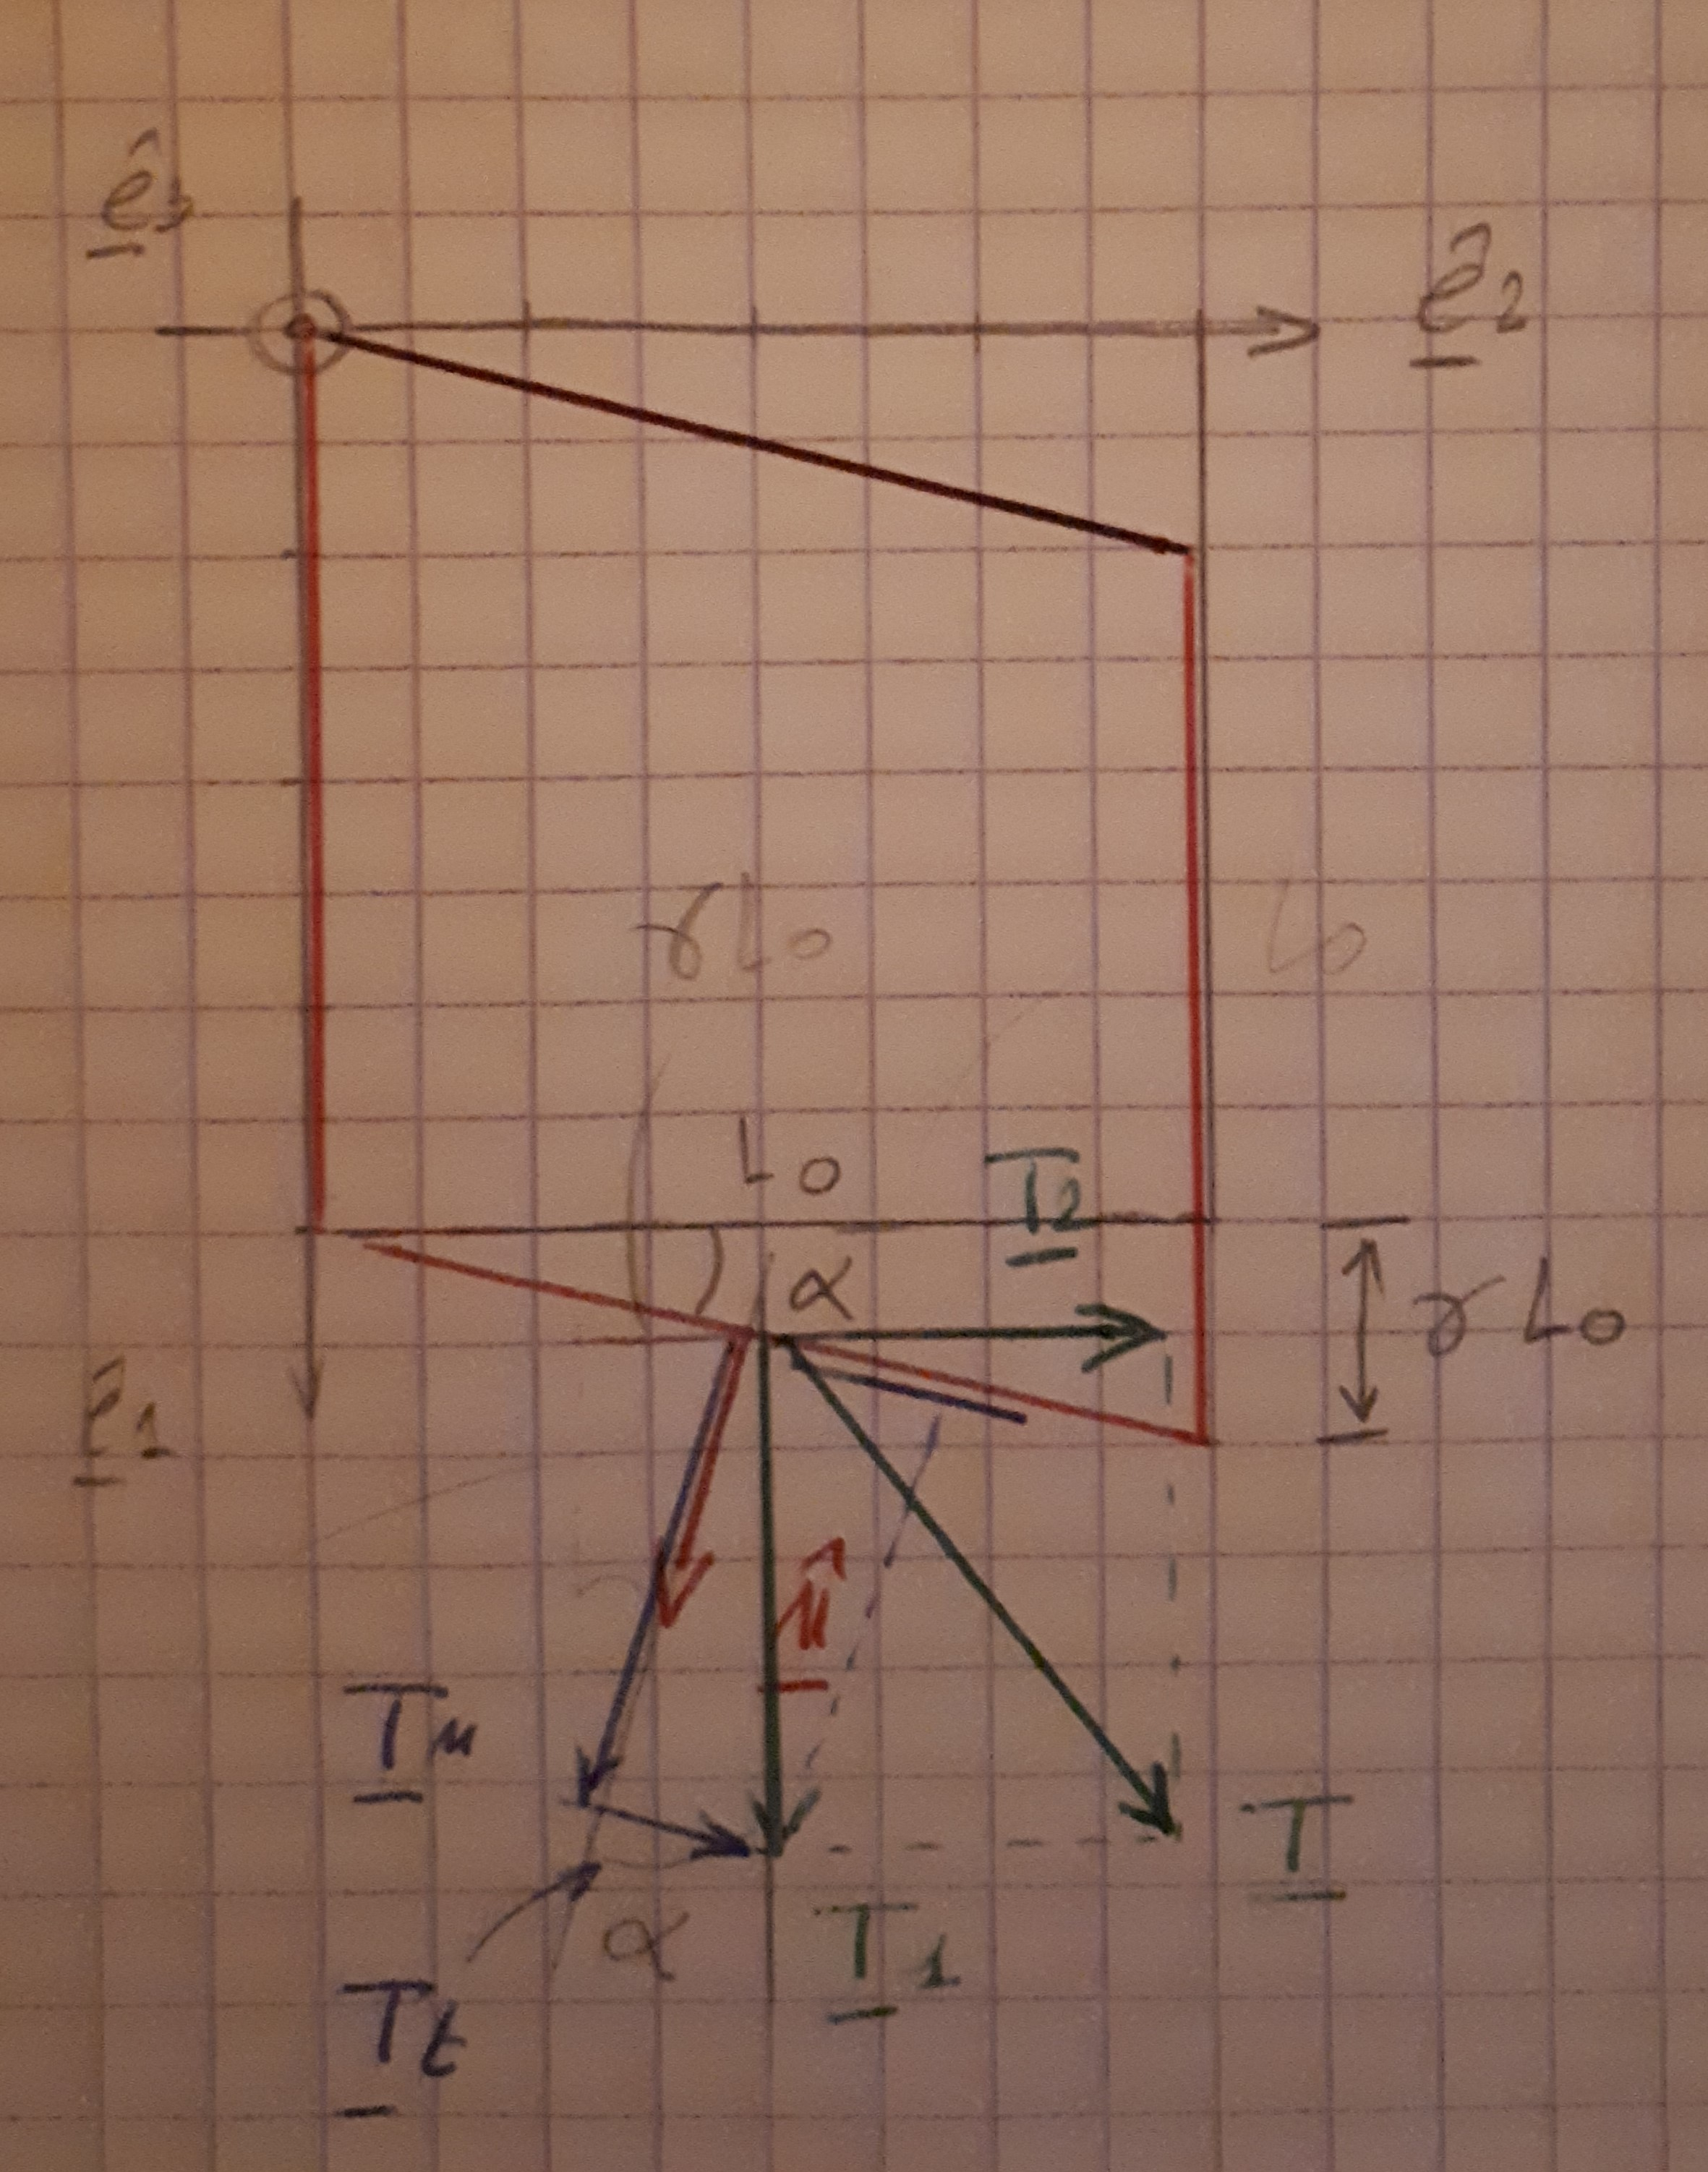
\includegraphics[width=0.5\textwidth]{MMC_Janvier_2019_Min_Q3_Image2.jpg}
\end{center}

L'orientation de la facette initialement en $X_1=L_0$ change par rapport à la configuration initiale.

Normale facette déformée : $\vec{\hat{n}}=\begin{pmatrix}cos\alpha \\ -sin\alpha \\ 0 \end{pmatrix} \ avec \ \alpha = arctg\left(\frac{\gamma L_0}{L_0}\right)= arctg \ \gamma$

Contrainte sur la facette : $\vec{T}(\vec{\hat{n}}) = \matr{\sigma}  \cdot  \vec{\hat{n}} =\begin{pmatrix}\mu (\frac{2\gamma^2}{3} \ cos \alpha- \gamma \ sin\alpha) \\ \mu (\gamma \ cos \alpha + \frac{\gamma}{3} \ sin \alpha) \\ 0 \end{pmatrix}$

Contrainte normale : $T_n=\vec{T}(\vec{\hat{n}})  \cdot  \vec{\hat{n}} = \frac{2\mu\gamma^2}{3} {cos}^2 \ \alpha-2\ \gamma \ sin\alpha \ cos\alpha-\frac{\gamma}{3}{sin}^2 \alpha$

Contrainte tangentielle : $T_t= \sqrt{T^2 - T^2_n}$

\textit{NdC : sur sa feuille avec les réponses, l'assistant à indiqué que la normale de la facette déformée était :}

\begin{equation*}
\vec{\hat{n}}=\frac{1}{\sqrt{1+\gamma^2}}\begin{pmatrix} 1 \\ -\gamma \\ 0 \end{pmatrix}.
\end{equation*}

\textit{Je ne comprends pas. Pour pouvoir écrire cela, il faut faire l'hypothèse que la déformation est petite, ce qui donne :}

\begin{equation*}
\alpha = \arctan \gamma \approx \gamma.
\end{equation*}

\textit{Mais ce n'est qu'au dernier point que l'on fait l'hypothèse des petites déformations.  Voici le reste des réponses de l'assistant :}

\begin{center}
$\vec{T}(\vec{\hat{n}})=\frac{1}{\sqrt{1+\gamma^2}}\begin{pmatrix} \frac{-\mu \gamma^2}{3} \\ \mu \gamma \left(1+\frac{\gamma^2}{3} \right) \\ 0 \end{pmatrix}$   ;   $T_n = \frac{-\mu \gamma^2}{3 (1+\gamma^2} \left(4+\gamma^2 \right)$   ;   $T_t = \frac{-\mu \gamma^2}{3 (1+\gamma^2})$
\end{center}

\textit{Petite remarque : bien faire attention que l'on demandait la contrainte sur la facette \textsc{déformée} : il faut donc calculer $\vec{T}$ à l'aide de la normale \textsc{unitaire} de la facette \textsc{déformée}, et non de $\vec{\hat{e}}_1$.}

\textbf{Réponse partie 2, sous-question 5}

$det \left(\matr{\sigma} - \lambda \matr{I} \right) =
\begin{bmatrix}
\frac{2 \mu \gamma^2}{3}-\lambda & \mu \gamma & 0 \\
\mu \gamma & -\frac{\mu \gamma^2}{3} - \lambda & 0 \\
0 & 0 & -\frac{\mu \gamma^2}{3} - \lambda \\
\end{bmatrix}
= \left( \frac{\mu\gamma^2}{3} + \lambda \right) \ \left(-{\lambda}^2+\frac{\mu\gamma^2}{3} \lambda - \frac{2{\mu}^2{\gamma}^4}{9}+{\mu}^2{\gamma}^2 \right)
=0
$

$\sigma_1 = \frac{\mu\gamma^2}{6} \left(1+3\sqrt{4+\gamma^2} \right)$ ; $\sigma_2 = \frac{-\mu\gamma^2}{3}$ ; $\sigma_3 = \frac{\mu\gamma^2}{6} \left(1-3\sqrt{4+\gamma^2} \right)$. 

\textit{NdC : sur sa feuille de réponse, l'assistant avait noté : $\sigma_{1,2} = \frac{\mu\gamma^2}{6} \left(1 \pm 3 \sqrt{ 1+\left(\frac{2}{\gamma}\right)^2} \right)$, mais je ne suis pas parvenu à retrouver cette expression.}

\textbf{Réponse partie 2, sous-question 6}

\begin{center}
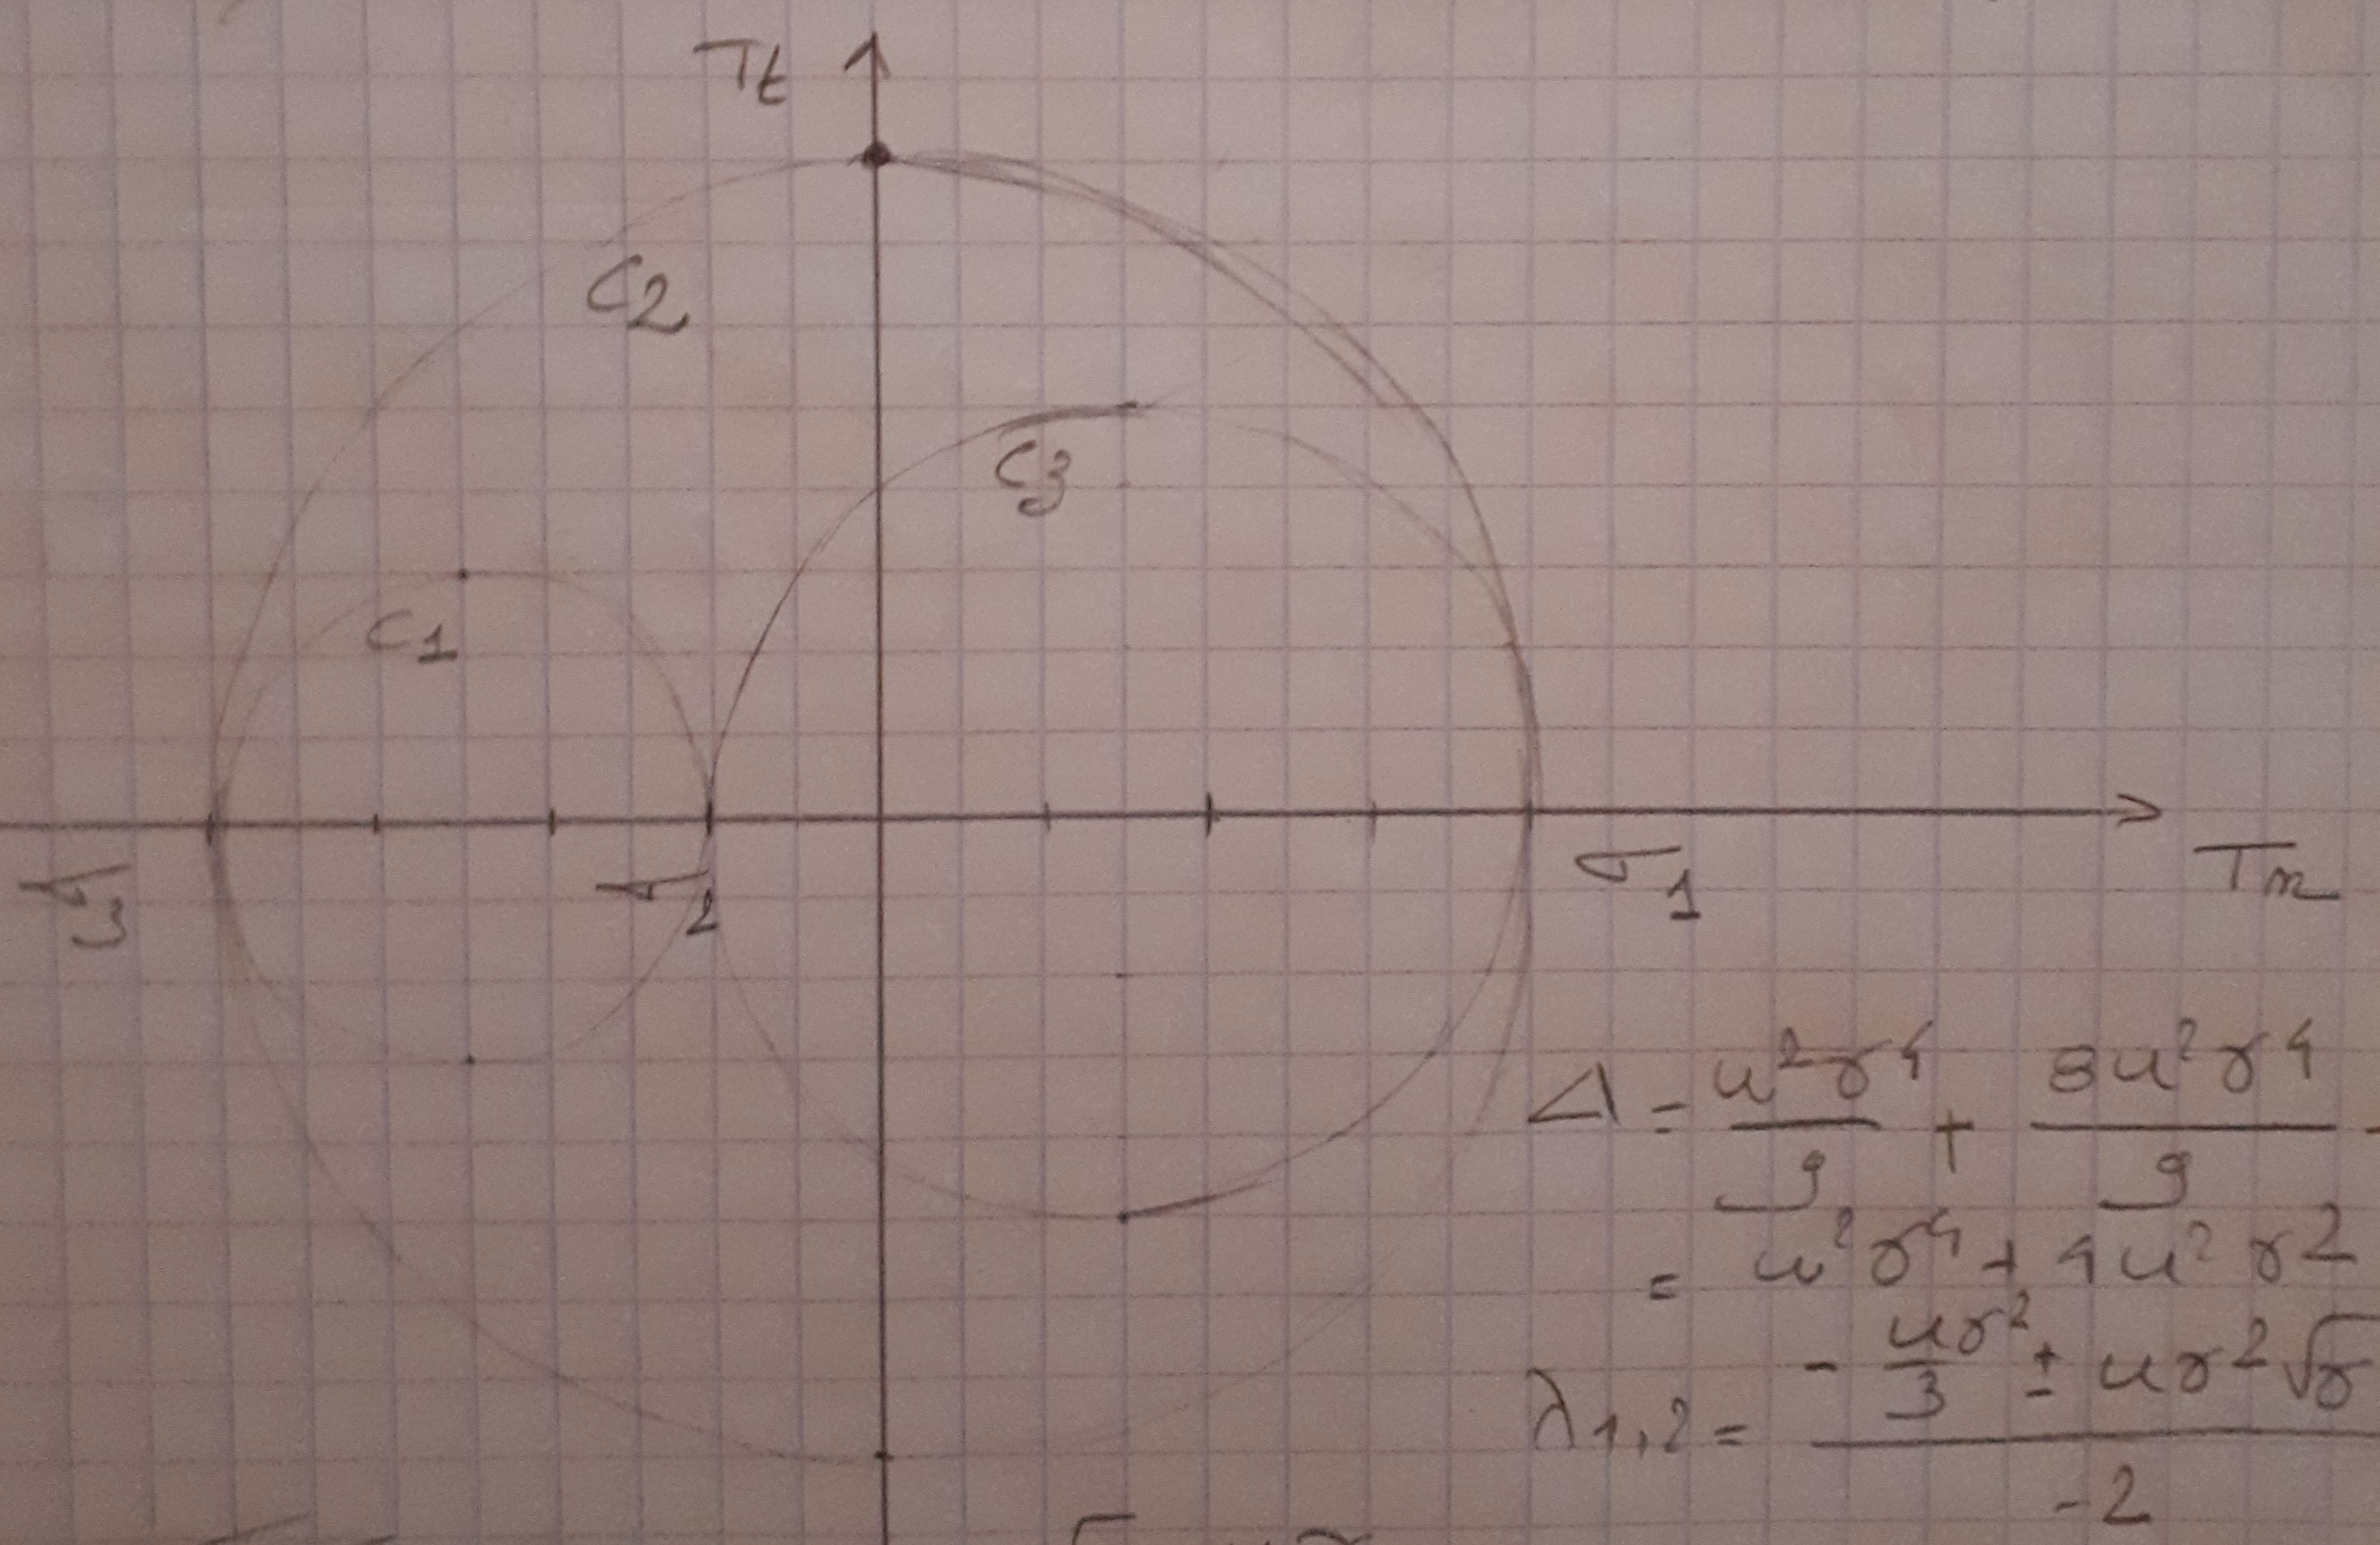
\includegraphics[width=0.5\textwidth]{MMC_Janvier_2019_Min_Q3_Image3.jpg}
\end{center}

Contrainte de cisaillement maximale : $T_{t \ max} = \frac{\sigma_1 - \sigma_3}{2} = \frac{\mu\gamma^2}{2}\sqrt{4+\gamma^2}$.

\textit{NdC : sur sa feuille de réponse, l'assistant avait noté : $\frac{\mu\gamma^2}{2}\sqrt{1+\left(\frac{2}{\gamma}\right)^2}$.}

\textbf{Réponse partie 2, sous-question 7}

$\matr{F} = \begin{pmatrix} 1 & \gamma & 0 \\ 0 &1 & 0 \\ 0 & 0 & 1 \end{pmatrix}$

$\matr{B} = \matr{F} \cdot \matr{F}^T = \begin{pmatrix} 1 & \gamma & 0 \\ \gamma & 1 & 0 \\ 0 & 0 & 1 \end{pmatrix}$

$\matr{\sigma} = \begin{pmatrix} 0 & \mu \gamma & 0 \\ \mu \gamma & 0 & 0 \\ 0 & 0 & 0 \end{pmatrix}$

$\vec{T}(\vec{\hat{e}}_2) = \begin{pmatrix} \mu \gamma & 0 & 0 \end{pmatrix}^T \ \Rightarrow \ T_n = 0 \ ; \ T_t = \mu \gamma$

$\vec{T}(\vec{\hat{n}}) = \begin{pmatrix} -\mu \gamma \ sin \alpha \\  \mu \gamma \ (cos \alpha + \frac{1}{3} sin\alpha) \\  0 \end{pmatrix}$

$\begin{bmatrix} -\lambda & \mu \gamma & 0 \\ \mu \gamma & -\lambda & 0 \\ 0 & 0 & -\lambda \end{bmatrix}=-\lambda \ \left(\lambda^2-\mu^2 \gamma^2 \right) = 0 \Rightarrow \ \sigma_1 = \mu\gamma$ ; $\sigma_2 = 0$ ; $\sigma_3 = -\mu\gamma$.

Cercles de Mohr : même chose qu'à la sous-question précédente, sauf que $\sigma_2 = 0$ et donc que les cercles $C_1$ et $C_3$ ont le même diamètre.  

$T_{t \ max} = \mu\gamma$

 \textit{NdC : pour la facette qui était en $x_1 = L_o$ (sous question 3.4, je n'ai pas recalculé $T_t$ ni $T_n$.  Un peu lourd ...  Les réponses n'étaient pas sur la feuille de l'assistant non plus.}

\end{solution}

%-------------------------------------------------------------------------
% FIN SOLUTION QUESTION 3
%-------------------------------------------------------------------------

\section{Application Fluide: écoulement visqueux d'un fluide newtonien autour d'un cylindre}

On étudie l'écoulement stationnaire d'un fluide visqueux newtonien incompressible et indilatable \textit{autour} d'un tube cylindrique de rayon $R$ (voir figure).  Le tube cylindrique est placé verticalement et le fluide s'écoule le long du cylindre sous l'unique action de la gravité.  On suppose que le tube cylindrique est infini et que l'écoulement est établi.  Le fluide [partie illisible sur la photo de l'énoncé] un film fin d'une épaisseur $h$ sur la face extérieure du cylindre.  La pression de l'atmosphère est uniforme et vaut $p_a$.  En outre, on néglige toute intercation visqueuse avec l'atmosphère.

On vous demande de :

\begin{enumerate}
    \item Poser les hypothèses semi-inverse sur la forme des champs de vitesse et de pression de l'écoulement.  Justifier et expliquer clairement chaque hypothèse.
    \item Ecrire les équations à résoudre pour les champs de pression et de vitesse en effectuant toutes les simplifcations nécessaires.
    \item Ecrire les différentes conditions aux frontières du problème.
    \item Résoudre les équations sans imposer encore les conditions frontières.  Mettre en évidence l'expression du champ de vitesse et du champ de pression.
    Indication : $\frac{\partial^2f}{\partial x^2}+\frac{1}{x} \frac{\partial^f}{\partial x}=\frac{1}{x} \frac{\partial}{\partial x} \left(x\frac{\partial f}{\partial x} \right) $
    \item Sur base des conditions frontières, déterminer l'expression finale des champs de pression et de vitesse.
    \item Esquisser la forme du profil de vitesse.
    \item En partant de sa définition, déterminer la contrainte de cisaillement qui s'applique sur la surface du tube ($\tau_w$).
    \item En partant cette fois-ci de la conservation de la quantité de mouvement sur un volume de contrôle, ré-obtenir l'expression obtenue à la question précédente.
    \item Ecrire l'intégrale à calculer pour obtenir le débit.
    \item \textbf{Bonus :} calculer le débit.
\end{enumerate}

%-------------------------------------------------------------------------
% DEBUT SOLUTION QUESTION 4 
%-------------------------------------------------------------------------

\begin{solution}

\textbf{Réponse sous-question 1}

\begin{center}
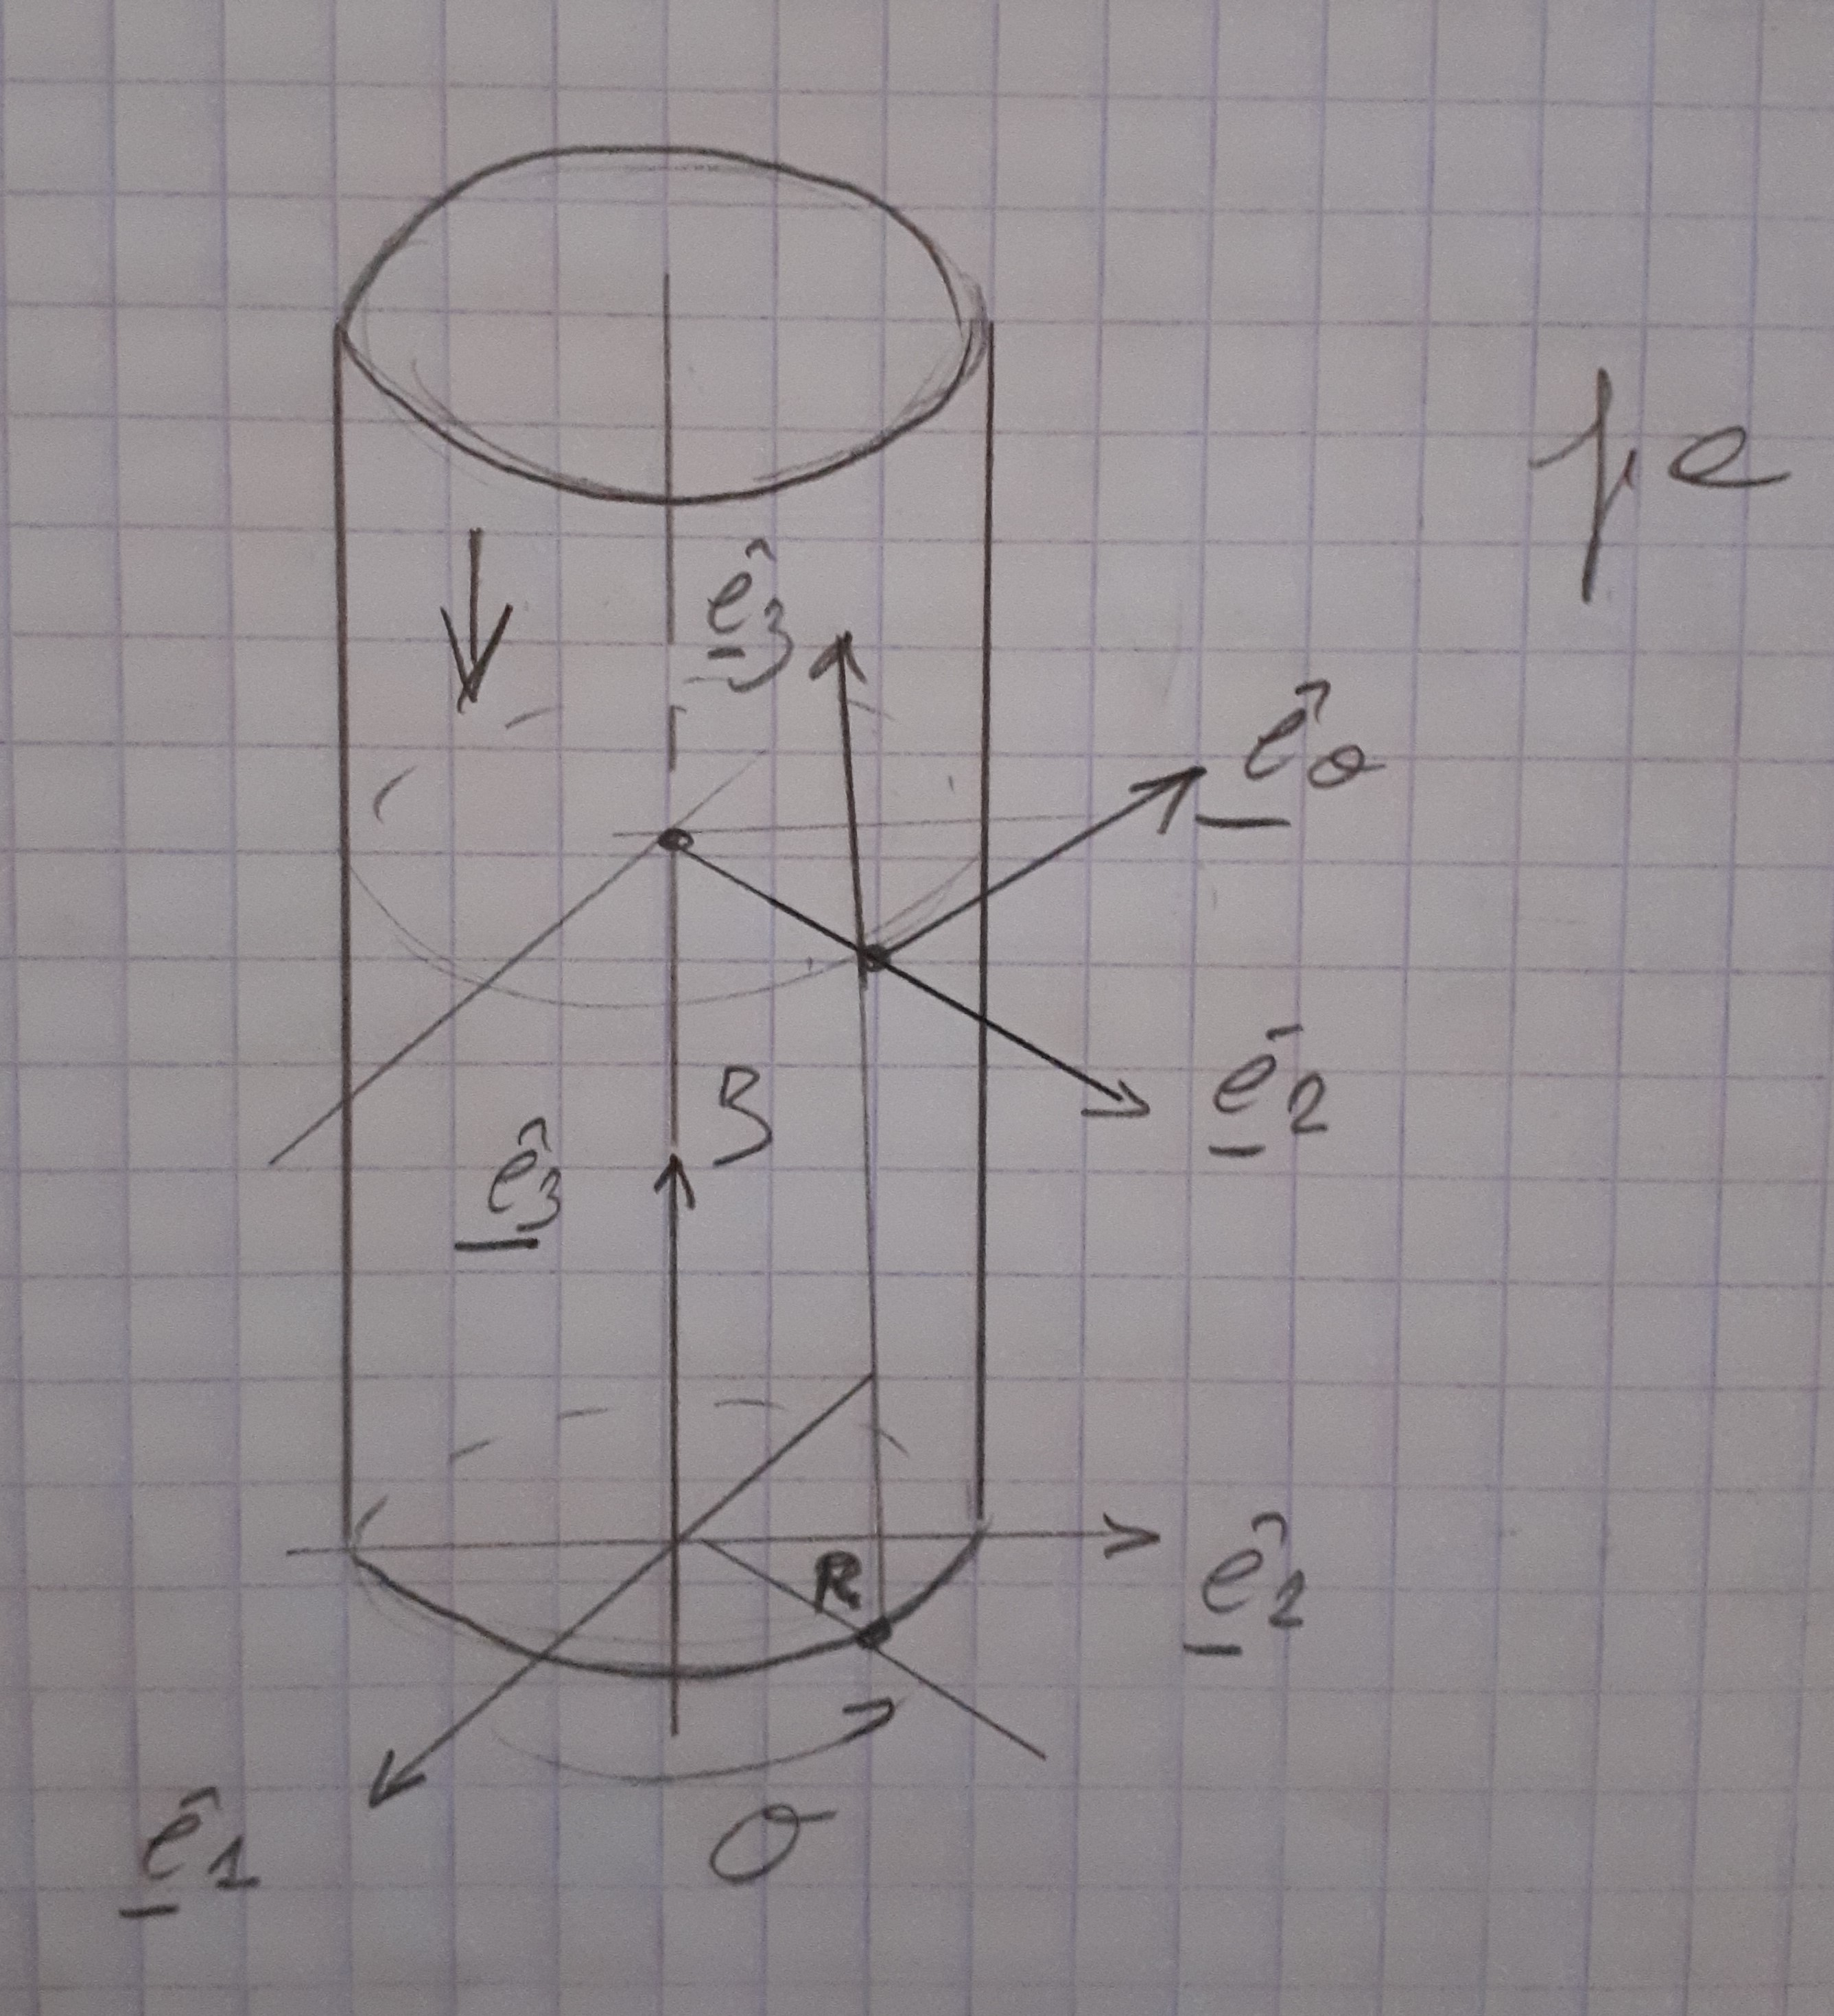
\includegraphics[width=0.5\textwidth]{MMC_Janvier_2019_Min_Q4_Image1.jpg}
\end{center}

$\vec{V}(r,\theta,z,t)=V_r(r,\theta,z,t) \ \vec{\hat{e}}_v + V_{\theta}(r,\theta,z,t) \ \vec{\hat{e}}_{\theta}+V_z(r,\theta,z,t) \ \vec{\hat{e}}_z$ \ $\Rightarrow \ \vec{V} = V_z(z) \ \vec{\hat{e}}_z$

Composantes :

\begin{itemize}
    \item $V_r$ : NON car hypothèse que le fluide suivant des lames cylindriques concentriques, et il n'y a rien dans l'énoncé qui laisse penser que le fluide pourrait sécouler suivant $\vec{\hat{e}}_r$.
    \item $V_{\theta}$ : NON car symmmétrique axiale et rien dans l'énoncé qui laisse penser que le fluide pourrait tourner autour du cylindre.
    \item $V_z$ : OUI car gravité.
\end{itemize}

Dépendance de $V_z$ :

\begin{itemize}
    \item $r$ : OUI car la vitesse a une valeur nulle à la paroi (fluide visqueux newtonien) et non nulle quand on s'écarte de la paroi.
    \item $\theta$ : NON car symmétrie axiale.
    \item $z$ : NON car fluide incompressible : si le fluide s'écoule suivant des lames cylindriques concentriques, les particules d'une même lame de fluide doivent toutes avoir la même vitesse.  Sinon, elles se rapprocheraient ou s'écarteraient, et la masse volumique du fluide varierait suivant $z$.  Or, le fluide est incompressible (énoncé).  On peut aussi le voir à l'aide de la forme locale du théorème de la conservation de la masse : pour un fluide incompressible, il donne :
    \begin{equation*}
        \text{div} \ \vec{V}
        = \frac{V_r}{r}
        +\frac{\partial V_r}{\partial r}
        + \frac{1}{\theta} \ \frac{\partial V_{\theta}}{\partial \theta}
        +\frac{\partial V_z}{\partial z} = 0 \ \Rightarrow \ \frac{\partial V_z}{\partial z} = 0
    \end{equation*}

    \item $t$ : NON car problème stationnaire.
\end{itemize}

$p = p(r,\theta,z,t) \ \Rightarrow \ p = p(r,z) \ ou \ p = p(z)$

Dépendances de p :

\begin{itemize}
    \item $r$ : pas encore d'idée.
    \item $\theta$ : NON car symmétrie axiale.
    \item $z$ : OUI car colonne de fluide, donc pression due à la colonne de fluide.
    \item $t$ : NON car problème stationnaire.
\end{itemize}

\textit{NdC : si à ce stade vous pensez que $p$ dépend uniquement de $r$, vous avez raison.  Ici, je joue le jeu en écrivant les dépendances que j'avais estimées être bonnes à ce stade de l'exercice et j'expliquerai comment, grâce aux calculs, on trouve que $p$ ne dépend que de $r$.  Je pense que ça pourrait aider les personnes pour qui ce n'est pas évident non plus.}

\textbf{Réponse sous-question 2}

$\rho \fDif{\vec{V}}{t} = \rho \vec{f}-\vec{\grad} \ p+\mu \ \Delta\vec{V}$

$\rho \frac{\partial \ \vec{V}}{\partial t} + \rho \left( \matr{\grad} \ \vec{V} \right) \cdot \vec{V} = \rho \vec{f}-\vec{\grad} \ p+\mu \ \Delta\vec{V}$

$\rho \left( \matr{\grad} \ \vec{V} \right) \cdot \vec{V} = \rho \vec{f} - \vec{\grad} \ p+\mu \ \Delta\vec{V}$

\textbf{Réponse sous-question 3}

$\vec{V} \ (r=R)=\vec{0}$

$p \ (r=R+h,z) = p_a$

\textbf{Réponse sous-question 4}

$\rho \left( \matr{\grad} \ \vec{V} \right) \cdot \vec{V} = \rho \vec{f}-\vec{\grad} \ p + \mu \ \Delta\vec{V}$

$\rho \begin{pmatrix} 0&0&0 \\ 0&0&0 \\ \frac{\partial V_z}{\partial r}&0&0 \end{pmatrix} \begin{pmatrix} 0 \\ 0 \\ V_z \end{pmatrix} = \begin{pmatrix} 0 \\ 0 \\ 0 \end{pmatrix} = \begin{pmatrix} 0 \\ 0 \\ -\rho g \end{pmatrix} + \begin{pmatrix} \frac{\partial p}{\partial r} \\ 0 \\  \frac{\partial p}{\partial z} \end{pmatrix} + \mu \begin{pmatrix} 0 \\ 0 \\ \frac{\partial^2V_z}{\partial r^2}+\frac{1}{r} \ \frac{\partial V_z}{\partial r} \end{pmatrix}$


\textit{NdC : la matrice utilisée ici pour représenter $\matr{\grad} \ \vec{V}$ est la transposée de celle donnée dans le formulaire.  La représentation dépend de la manière de réaliser le produit contracté.  La représentation utilisée dans cette correction est valable si on effectue une contraction $(2,3)$, qui correspond au produit d'une matrice $(3,3)$ par un vecteur $(3,1)$.  La matrice du formulaire représente le gradient si on effectue une contractaction $(1,3)$, qui correspond au produit matriciel d'un vecteur $(1,3)$ par une matrice $(3,3)$, qui sont tous les deux les transposés du vecteur et de la matrice de la contraction $(2,3)$.  Voir tableau ci-dessous.}

\begin{center}
\begin{tabular}{|c|c|c|}
    \hline
    Contraction & Représentation indicielle & Représentation matricielle \\
    \hline
    \rule{0pt}{25pt} (2,3) & $\left[ \left( \matr{\grad} \ \vec{V} \right) \cdot \vec{V} \right]_i = \left( \matr{\grad} \ \vec{V} \right)_{ij} V_j$ & $\left( \matr{\grad} \ \vec{V} \right) \cdot \left( \vec{V} \right)$ \\
    \hline
    \rule{0pt}{25pt} (1,3) & $\left[ \left( \matr{\grad} \ \vec{V} \right) \cdot \vec{V} \right]_i = \left( \matr{\grad} \ \vec{V}  \right)_{pi} V_p$ & $\left( \vec{V} \right)^T \cdot \left( \matr{\grad} \ \vec{V} \right)$ \\
    \hline
\end{tabular}
\end{center}

Suivant $\vec{\hat{e}}_r$ : $\frac{\partial p}{\partial r}=0$.

$p$ ne dépendrait donc que de $z$.  Mais on a la condition limite $p(r=R+h,z) = p_a$, qui devient $p(z) = p_a$.  Or, $p_a$ est une constante (énoncé~: la pression atmosphérique est uniforme).  Donc, $p$ ne dépend pas non plus de $z$.

$\Rightarrow$ $p \ = \ p_a$

Suivant $\vec{\hat{e}}_z$ : $\rho g - \mu \frac{\partial^2V_z}{\partial r^2} - \mu \frac{1}{r} \frac{\partial V_z}{\partial r} = 0$

On utilise l'indication donnée dans l'énoncé : $\mu \frac{1}{r} \frac{\partial}{\partial r} \left(r \ \frac{\partial V_z}{\partial r} \right) = \frac{\rho g}{\mu} r$ 

$r \frac{\partial V_z}{\partial r} = \frac{\rho g}{\mu} \frac{r^2}{2} + \frac{K_1}{r}$

=> $V_z = \frac{\rho g}{4 \mu} r^2 + K_1 \ ln(r) \ + K_2$

\textbf{Réponse sous-question 5}

En $r=R$ : $\vec{V}=\vec{0}$

$\frac{\rho g}{4 \ mu} r^2 + K_1 \ ln(R) \ + K_2$

En $r=R+h$ : $p \ (r=R+h,z) = p_a$ , soit $\vec{T} \  (\vec{\hat{n}}=\vec{\hat{e}}_r, \ r = R+h) = \begin{pmatrix} -p_a&0 &0 \end{pmatrix}^T$

$\matr{D} = \frac{1}{2} \left[ \left( \matr{\grad} \ \vec{V} \right) + \left( \matr{\grad} \ \vec{V} \right)^T\right] = \begin{pmatrix}
0 & 0 & \mu \frac{\partial V_z}{\partial r} \\
0 & 0 & 0 \\
 \mu \frac{\partial V_z}{\partial r} & 0 & 0
\end{pmatrix}$

$\matr{\sigma} = 2 \mu \ \matr{D} + \lambda \ tr(\matr{D}) \ \matr{I} - p \ \matr{I} = \begin{pmatrix} -p & 0 & \mu \frac{\partial V_z}{\partial r}\\ 0 & -p & 0 \\ \mu \frac{\partial V_z}{\partial r} & 0 & -p \end{pmatrix}$

$\vec{T} \ (\vec{\hat{n}}=\vec{\hat{e}}_r, \ r = R+h) = \matr{\sigma} \cdot \ \vec{\hat{e}}_r = \begin{pmatrix} -p & 0 & \mu \frac{\partial V_z}{\partial r} \\ 0 & -p & 0 \\ \mu \frac{\partial V_z}{\partial r} & 0 & -p \end{pmatrix} \ \begin{pmatrix} -1\\0\\0 \end{pmatrix} = \begin{pmatrix} -p \\ 0 \\ \mu \frac{\partial V_z}{\partial r}\end{pmatrix} $

Suivant $\vec{\hat{e}}_r$ : $p = p_a$ (déjà trouvé au point 4)

Suivant $\vec{\hat{e}}_z$ : $\left(\mu \frac{\partial V_z}{\partial r} \right)_{r=R+h} = \frac{\rho g}{2 \ \mu} \ (R+h) + \frac{K_1}{R+h} = 0$

=> $K_1 = -\frac{\rho g}{2 \mu} (R+h)^2$ 

=> $K_2 = -\frac{\rho g}{4 \mu} R^2 + \frac{\rho g}{2 \ \mu} (R+h)^2 \ ln(R)$ 

=> $V_z = \frac{\rho g}{\mu} \left(\frac{r^2-R^2}{4} - \frac{(R+h)^2}{2} \ ln\left(\frac{r}{R}\right) \ \right)$

\textbf{Réponse sous-question 6}

Allure de $V_z \ (r)$ ?

$V_z \ (r=R) = 0$ (OK car fluide visqueux newtonien).

$\frac{\partial V_z}{\partial r} = \frac{\rho g}{\mu} \left( \frac{r}{2} - \frac{(R+h)^2}{2} \ \frac{1}{r} \right)$

$\left( \frac{\partial V_z}{\partial r} \right)_{r=R} = \frac{\rho g}{\mu} \left( \frac{-h^2-2Rh}{2R}\right) < 0$

Le signe négatif est-il logique ?  Logiquement, la vitesse du fluide doit augmenter lorsque l'on s'éloigne de la paroi.  Comme $\vec{\hat{e}}_z$ est dirigé vers le haut,$V_z$ est négative.  Le signe négatif signifie que lorsque l'on est à la paroi ($V_z=0$) et que l'on s'en écarte, la vitesse diminue, c'est à dire qu'elle devient négative.  Le signe semble donc cohérent.

$\left( \frac{\partial V_z}{\partial r} \right)_{r=R+h} = \frac{\rho g}{\mu} \left( \frac{R+h}{2} - \frac{R+h}{2}\right) = 0$

$\frac{\partial^2 V_z}{\partial r^2} = \frac{\rho g}{\mu} \left( \frac{1}{2}+\frac{(R+h)^2}{4}\frac{1}{r^2}\right) > 0$ \ $\Rightarrow$ \ Concavité vers le haut.

\begin{center}
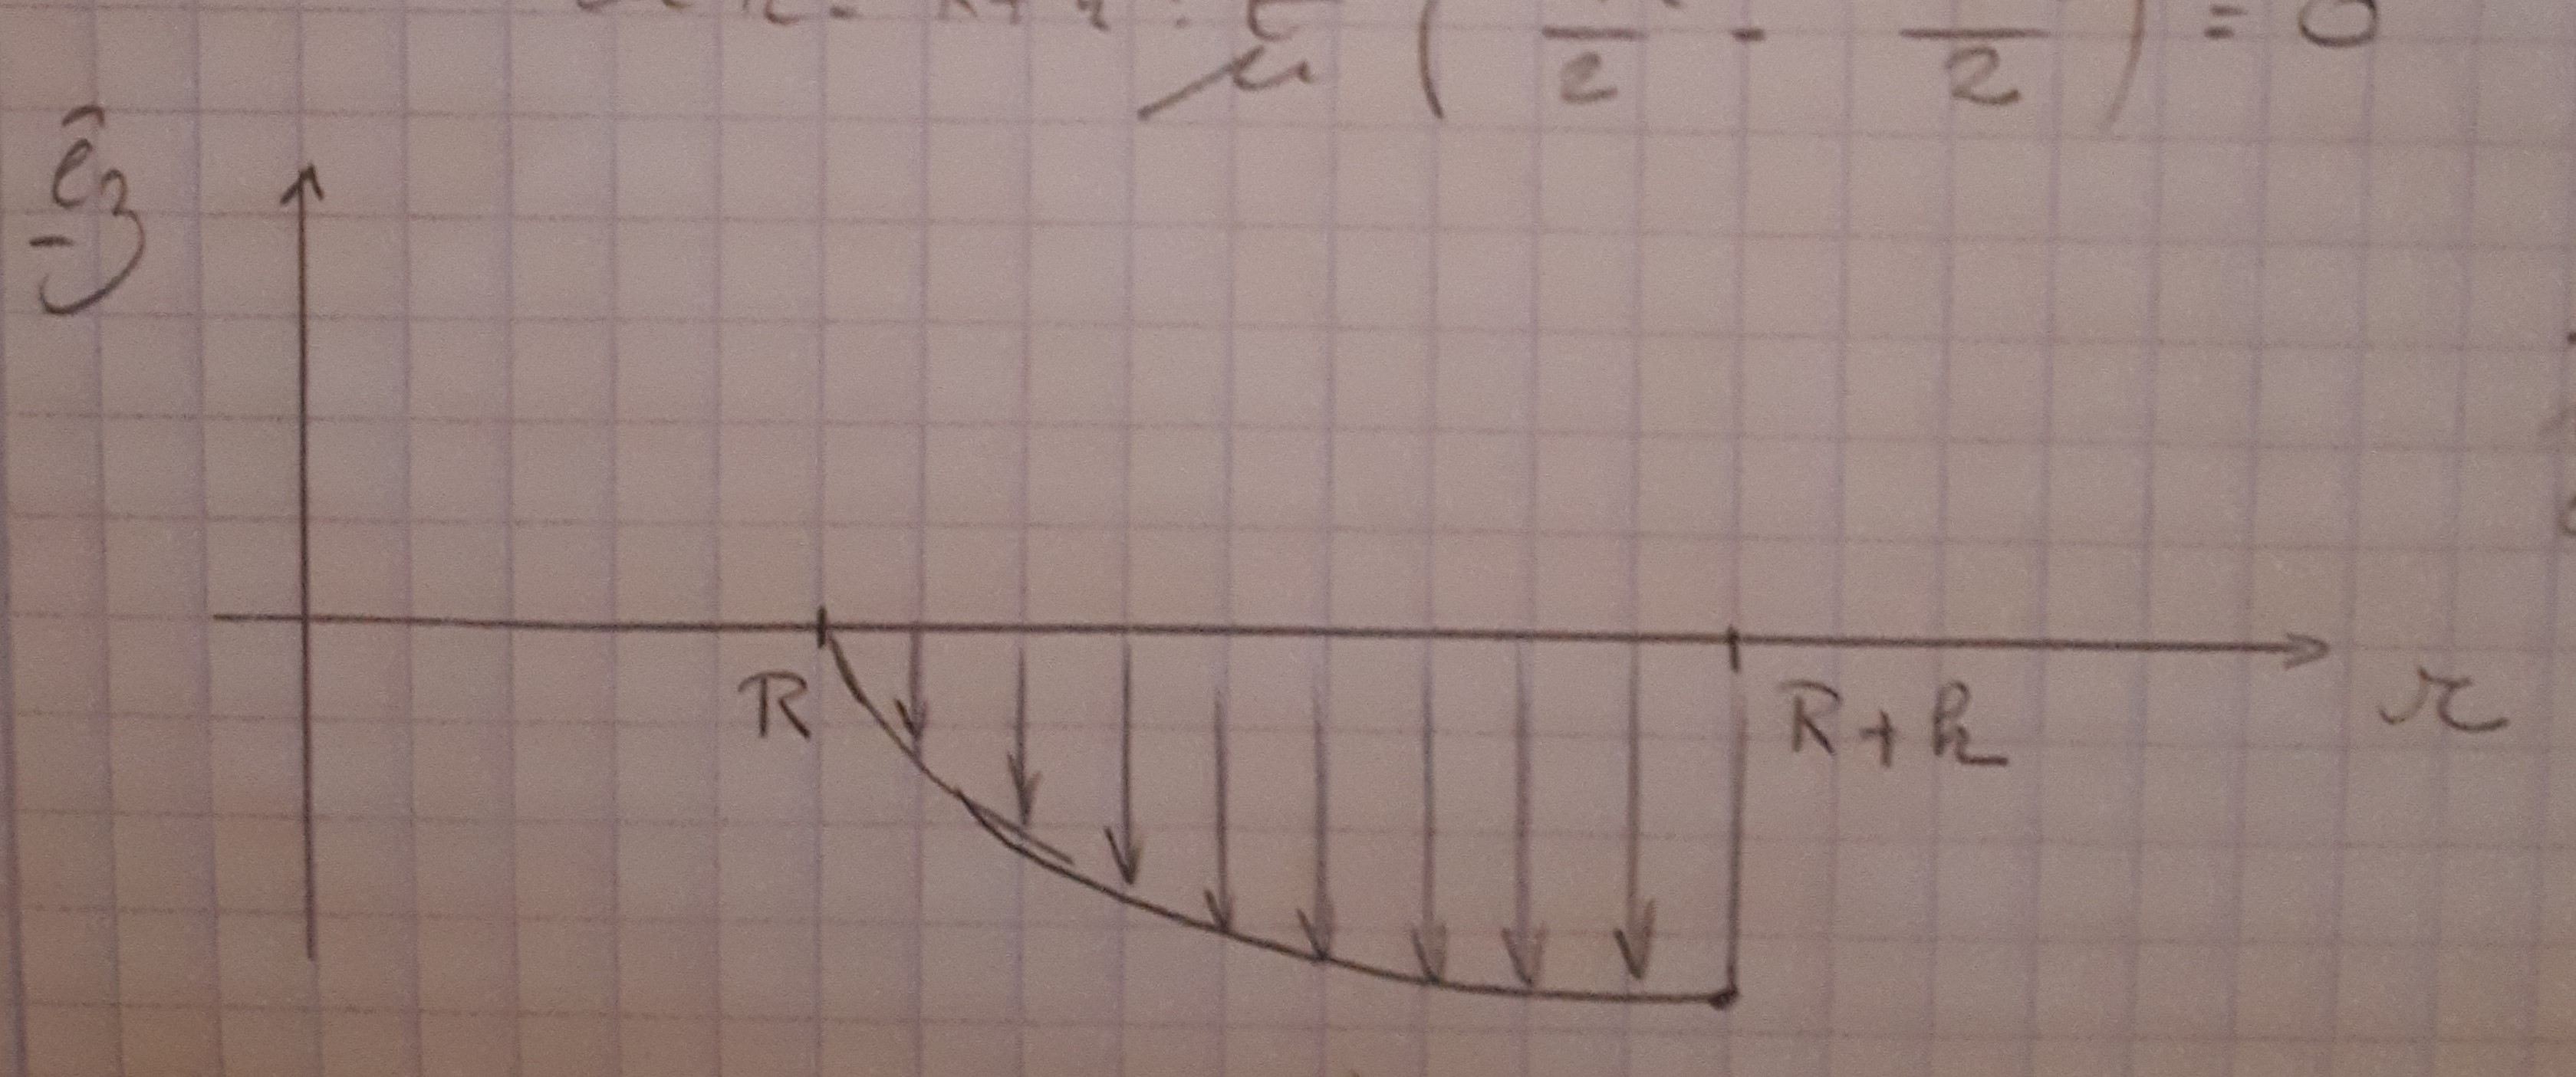
\includegraphics[width=0.5\textwidth]{MMC_Janvier_2019_Min_Q4_Image2.jpg}
\end{center}

\textit{NdC : lors de la consultation des copies, l'assistant m'a dit qu'il m'avait enlevé des points parce que les pente du profil en $r=R$ et en $r=R+h$ n'étaient pas correctes.  J'avais tracé à l'arrache.  Veillez donc à représenter, sur votre esquisse, les caractéristiques importantes du profil : valeur nulle et pentes.  Je ne sais pas s'ils tiennent compte de la concavité, car je ne me souviens plus si l'assistant avait fait une remarque ou pas.}

\textbf{Réponse sous-question 7}

$\tau_w = \left( \sigma_{rz} \right)_{r=R} = \left( \mu \frac{\partial V_z}{\partial r} \right)_{r=R} = -\rho g \left( \frac{h^2+2Rh}{2R} \right)$

\textbf{Réponse sous-question 8}

$\frac{\delta}{\delta t}  \displaystyle{\int_{\Delta t}} \rho \vec{V} \ dv +  \displaystyle {\int_{\Sigma t}} \rho \vec{V} \  (\vec{V} - \vec{W}) \cdot \vec{\hat{n}} \ dS = \vec{F} = \displaystyle{\int_{\Delta t}} \rho \ \vec{f} \ dv + \displaystyle{\int_{\Sigma t}} \vec{T} \ dS$

\textit{NdC : les symboles utilisées dans la formule ci-dessus, $\delta$, $\Delta t$ et $\Sigma t$, sont ceux du livre Mécanique des Milieux Continus, 4ème édition, de Jean Coirier et Carole Nadot-Martin, édition Dunod, pour un volume de contrôle.}

Le volume de contrôle est fixe $\Rightarrow \ \vec{W} = \vec{0}$.

L'écoulement est en régime stationnaire, ce qui signifie qu'en un point donné, les grandeurs (vitesse, pression, ...) sont constantes $\Rightarrow$ La quantité de mouvement contenue dans le volume de contrôle $\Delta t$ (ou $\Delta$, car volume de contrôle fixe, et donc indépendant du temps) est constante $\Rightarrow \frac{\delta}{\delta t} ... = 0 $.

Surfaces latérales ($r=R$ avec $\vec{\hat{n}}=-\vec{\hat{e}}_r$ et $r=R+h$ avec $\vec{\hat{n}}=\vec{\hat{e}}_r$) : $\vec{V} \ \bot \ \vec{\hat{e}}_r \ \Rightarrow$ l'intégrale de flux sur les surfaces latérales est nulle.

Surface annulaire supérieure ($r : R \rightarrow R+h$ avec $\vec{\hat{n}}=\vec{\hat{e}}_z$) : $\vec{V} \ \vec{V} \cdot \vec{\hat{n}} = V_z^2 \ \vec{\hat{e}}_z$.

Surface annulaire inférieure ($r : R \rightarrow R+h$ avec $\vec{\hat{n}}=-\vec{\hat{e}}_z$) : $\vec{V} \ \vec{V} \cdot \vec{\hat{n}} = V_z^2 \ \vec{\hat{e}}_z$.

\textit{NdC : je me suis arrêté là et je n'ai pas calculé les intégrales.  Désolé.}


\textbf{Réponse sous-question 9}

$\dot{m} = \displaystyle{\int_{\Sigma t}} \rho \ \vec{V} \cdot \vec{\hat{n}} \ dS = \displaystyle{\int_{\Sigma t}} \rho \ V_z \ dS$

\textbf{Réponse sous-question 10}

\nosubsolution


\end{solution}

%-------------------------------------------------------------------------
% FIN SOLUTION QUESTION 4
%-------------------------------------------------------------------------


\end{document}
